\section{User Testing}
My goal for the user testing is to determine the intuitiveness and clarity of the website and to identify any issues.
As for the target user group, I have chosen developers.

I have created the following scenarios for the user testing:
\begin{itemize}
    \item Common Format Generation from Proto Files
    \item List Services, Methods, Message Types, and Enum Types
    \item Comments and Options
    \item Execute Unary Request
    \item Execute Server Streaming Request
    \item Complex Method Input
    \item Global Metadata
\end{itemize}

The scenarios are different from those for testing the functionality of the website
and do not cover the entire functionality
because the primary goal of user testing is the intuitiveness and clarity of the website.

Each user will be briefed about the website's general use-case,
asked about their experience with similar pieces of software,
and then they will be asked to complete the scenarios
and provide feedback on the website's functionality and clarity.

The pre-questionnaire will be used to gather information about the user's experience with similar software.
The questions are:
\begin{itemize}
    \item What is your main focus in programming?
    (software, hardware, web development, etc.)
    \item What is your experience with REST APIs or GraphQL?
    \item What is your experience with Swagger UI, GraphiQL, or similar tools?
    \item What is your experience with the gRPC?
\end{itemize}

The post-questionnaire will be used to gather feedback on the website's functionality and clarity.
The questions are:
\begin{itemize}
    \item How did you find the common format generation process?
    (rate 1--5, 1 being the best)
    \item How did you find the overall website design?
    (rate 1--5, 1 being the best)
    \item How difficult was to find the methods, message types, and enums?
    (rate 1--5, 1 being the easiest)
    \item How difficult was to control the method execution?
    (rate 1--5, 1 being the easiest)
    \item Is there anything else to add?
\end{itemize}

\subsection{Common Format Generation from Proto Files}
The tester is provided with proto files and a script for generating a common format with its documentation.

\textbf{The following instructions are given:}\\
Based on the provided proto files, generate a common format which will be used later on for the documentation website.

\textbf{The expected result is:}\\
A generated common format JSON file.

\subsection{List Services, Methods, Message Types, and Enum Types}
The tester is provided with the common format file.
The website is running on localhost on port 3000.

\textbf{The following instructions are given:}\\
You have a website running on the localhost on port 3000.
List all services, methods, message types, and enum types from the common format file.
Find the method \texttt{SayHello} and tell me what type it gives as a response.

\textbf{The expected result is:}\\
The method is found and the type is \texttt{HelloReply}.

\subsection{Comments and Options}
The tester is provided with the common format file.
The website is running on localhost on port 3000.

\textbf{The following instructions are given:}\\
You have a website running on the localhost on port 3000.
What does the method \texttt{ListFeatures} in the service \texttt{RouteGuide} do, and what is the \textit{java\_package} of that service?

\textbf{The expected result is:}\\
The method obtains features within the given rectangle and the \textit{java\_package} is \textit{guiding.route}.

\subsection{Execute Unary Request}
The tester is provided with the common format file.
The website is running on localhost on port 3000, and the gRPC-Web proxy with gRPC server is set up.

\textbf{The following instructions are given:}\\
You have a website running on the localhost on port 3000.
Execute method \texttt{SayHello} with their parameters and tell me the response with their headers and trailers.

\textbf{The expected result is:}\\
The method is executed with any parameter
and the response is \enquote{Hello Name} in the \texttt{message} field of the response message type.

\subsection{Execute Server Streaming Request}
The tester is provided with the common format file.
The website is running on localhost on port 3000, and the gRPC-Web proxy with gRPC server is set up.

\textbf{The following instructions are given:}\\
You have a website running on the localhost on port 3000.
Execute method \texttt{SayRepeatHello} with their parameters and tell me the responses with their headers and trailers.

\textbf{The expected result is:}\\
The method is executed with any parameter
and the response is \enquote{Hello Name} multiple times in the \texttt{message} field of the response message type.

\subsection{Complex Method Input}
The tester is provided with the common format file.
The website is running on localhost on port 3000, and the gRPC-Web proxy with gRPC server is set up.

\textbf{The following instructions are given:}\\
You have a website running on the localhost on port 3000.
Execute method \texttt{ListFeatures} with their parameters and tell me the responses.
The parameters are the following:
\begin{itemize}
    \item \texttt{lo}: latitude: 400000000, longitude: -750000000,
    \item \texttt{hi}: latitude 420000000, longitude -73000000.
\end{itemize}

\textbf{The expected result is:}\\
The method is executed with the parameters and responses are returned.

\subsection{Global Metadata}
The tester is provided with the common format file and authorization token.
The website is running on localhost on port 3000, and the gRPC-Web proxy with gRPC server is set up.

\textbf{The following instructions are given:}\\
You have a website running on the localhost on port 3000.
Execute method \texttt{SayHello} with the authorization token.

\textbf{The expected result is:}\\
The method is executed, and in the request metadata section, the authorization token is present.

\subsection{Testing Results}
The testing has been conducted with five developers, regardless of their experience with gRPC\@.
The goal was to determine the intuitiveness and clarity of the website and to identify any issues.
The individual testing reports follow in the next sections.

\subsubsection{Tester 1}
\textbf{Pre-questionnaire answers:}
The first tester is a bachelor's degree student in computer science.

\begin{enumerate}
    \item Mobile applications and hardware.
    \item Using them every day.
    \item Using them at work for documentation, checking and testing the APIs.
    \item Heard of, but never used.
\end{enumerate}

\textbf{Post-questionnaire answers:}
\begin{enumerate}
    \item 1 -- It is clear and simple to use, but he would prefer to have a button for the generation in the UI\@.
    \item 2 -- Good, clear overview.
    The metadata button is not clear, it feels like submitting the row.
    \item 1 -- All good.
    \item 1 -- All clear, familiar design and controls ti the Swagger UI\@.
    \item No.
\end{enumerate}

\textbf{Individual scenarios:}
\begin{enumerate}
    \item All done as expected.
    \item All done as expected.
    \item All done as expected.
    \item The first method execution was done without any parameters (that is acceptable by gRPC, so it is not an issue).
    The rest was done as expected.
    \item All was done as expected.
    He did not expect the number after a name in the response message (not part of my implementation, it is related to the backend).
    \item All done as expected.
    \item All done as expected.
\end{enumerate}

\subsubsection{Tester 2}
The second tester is a bachelor's degree student in computer science.

\textbf{Pre-questionnaire answers:}
\begin{enumerate}
    \item Web development, full-stack.
    \item Using them actively.
    \item Rarely used, but when used, he uses them for documentation and API design checking.
    The testing of endpoints is usually done using Postman.
    \item None.
\end{enumerate}

\textbf{Post-questionnaire answers:}
\begin{enumerate}
    \item 1 -- All was clear.
    \item 1 -- All clear, similar to Swagger UI\@.
    The only complaint is that the red color in client streaming invokes there is an error.
    \item 1 -- All was clear.
    \item 1 -- All was clear.
    \item He would expect the metadata button also in the method request, but he does not know how it is done in Swagger UI\@.
    (He has found it very quickly though.)
\end{enumerate}

\textbf{Individual scenarios:}
\begin{enumerate}
    \item All done as expected.
    \item He could not say the returned message type frame is the returned type.
    But he guessed the correct place quickly without any help.
    \item All done as expected.
    \item When he executed the method, he thought the request shown body was the response body.
    The rest was done as expected.
    \item The execution was done as expected.
    The only confusion was that he was not sure if the responses are a one returned list response, or multiple responses.
    He has suggested adding a title to each response.
    \item He could not find the input for the \texttt{lo} parameter before executing the method.
    This was caused by him playing with the application previously and accidentally changing the tab to the model.
    After pointing him to the correct tab, he found the input and the rest was done as expected.
    It was more of the testing preparation issue than the application issue connected with the stress from being a tester.
    \item All done as expected.
\end{enumerate}

\subsubsection{Tester 3}
The third tester is a bachelor's degree student in computer science.

\textbf{Pre-questionnaire answers:}
\begin{enumerate}
    \item Software development, management, and mobile development.
    \item Using REST APIs for mobile and web applications.
    Also using GraphQL web applications.
    \item None experience with Swagger UI\@.
    Some experience with Apollo Studio (not much though).
    \item None.
\end{enumerate}

\textbf{Post-questionnaire answers:}
\begin{enumerate}
    \item 1 -- All was clear.
    \item 2 -- Server streaming responses were too long, so the page becomes too long.
    The suggestion is to add scrolling, or a max height, or collapse the responses.
    The rest was clear.
    \item 1 -- All was clear.
    \item 1 -- All was clear.
    \item He would add the metadata button also in the method request, not only globally.
\end{enumerate}

\textbf{Individual scenarios:}
\begin{enumerate}
    \item All done as expected.
    \item All done as expected.
    \item All done as expected.
    \item When he executed the method, he thought the request shown body was the response body.
    The rest was done as expected.
    \item All done as expected.
    \item All done as expected, but when he had sent the request, he was waiting for the loading on the executed button to end.
    So he did not see the responses as they were coming.
    \item He could not find the global metadata settings because he did not connect metadata with authorization.
    The rest was done as expected.
\end{enumerate}

\subsubsection{Tester 4}
The fourth tester is a software developer with a master's degree in computer science.

\textbf{Pre-questionnaire answers:}
\begin{enumerate}
    \item Web engineering, backend development in Typescript.
    \item Everyday.
    \item Not much usage, but he knows what are they.
    He uses the Open API specification for REST APIs instead of Swagger UI\@.
    \item He was using it about 2 years ago for mobile development.
\end{enumerate}

\textbf{Post-questionnaire answers:}
\begin{enumerate}
    \item 1 -- All was clear.
    \item 1 -- Similar to Swagger UI, so all was clear.
    \item 1 -- He was not sure about the returned type model, the rest was clear.
    \item 1 -- He was looking a while for the button to execute the method, but he missed it because it was too wide.
    The rest was clear.
    \item If the gRPC API was larger, it would be good to have collapsible services/types/enums sections.
\end{enumerate}

\textbf{Individual scenarios:}
\begin{enumerate}
    \item All done as expected.
    \item He could not say if the returned type is the message body or the whole message type.
    But he had eventually remembered it is the whole message type.
    The rest was done as expected.
    \item All done as expected.
    \item He could not find the execution button because it was too long and he thought it was a heading.
    But he had eventually found it.
    The rest was done as expected.
    \item All done as expected.
    \item All done as expected.
    \item He was looking for metadata in the method, but quickly found it at the top.
    He has suggested making the button or header sticky at the top.
    He has also pointed out that the Bearer prefix addition seems unnecessary as there might be other types of authorization which this might not work with.
    The rest was done as expected.
\end{enumerate}

\subsection{Found Issues and Their Solutions}\label{subsec:found-issues-and-their-solutions}
The overall feedback was positive, and the testers found the website intuitive and clear.
However, few issues were found, and they are listed in the table~\ref{tab:user-testing-issues} with their respective solutions.
The changes are shown in the figure~\ref{fig:testing-screenshots}.

\newpage

\begin{table}[!htb]
    \centering
    \resizebox{\columnwidth}{!}{%
        \begin{tabular}{|p{0.4\linewidth}|p{0.4\linewidth}|l|}
            \hline
            Issue & Solution & State \\
            \hline
            The metadata button does not show a clear connection with authorization.
            & Renamed the button to \enquote{Metadata \& Authorization} (\ref{fig:testing-changes-top-bar}).
            & Fixed \\
            \hline
            The metadata button invokes the feeling of submitting the row (not opening a modal).
            & Added greater space between the button and the input fields.
            Also, making the input fields smaller, so the button is much larger.
            (\ref{fig:testing-changes-top-bar})
            & Fixed \\
            \hline
            Swapping the request with the response after the method execution.
            & Changed the request background color to white to match the metadata and highlight the heading.
            & Fixed \\
            \hline
            The metadata is expected also in the method execution.
            & Having only global metadata is a design decision based on the Swagger UI.
            The idea behind it is that the metadata is usually the same for all methods, carrying, for example, authorization.
            & Will not fix \\
            \hline
            The red color background in client streaming invokes there is an error.
            & The background colors have been redone to be lighter.
            Also, the client streaming color was changed to yellow.
            (\ref{fig:testing-changes-background-colors})
            & Fixed \\
            \hline
            Hard to distinguish the returned message type from the message type body.
            & Added description of the response status code and the title for the returned message type.
            (\ref{fig:testing-changes-response})
            & Fixed \\
            \hline
            Confusion if the responses are a response as a list, or a list of responses.
            & Added a title to each response with the message number and total count at the end.
            (\ref{fig:testing-changes-responses})
            & Fixed \\
            \hline
            Server streaming methods can have too many responses, so the page becomes too long.
            & The responses are now scrollable in a fixed height container.
            (\ref{fig:testing-changes-responses})
            & Fixed \\
            \hline
            Not seeing the responses as they are coming, waiting for the loading on the executed button to end.
            & Relocated the cancel button to the right side of the execution button.
            Changed the responses to be shown in a fixed height container.
            (\ref{fig:testing-changes-cancel})
            Also, this was more related to the tester's stress, where in reality they would scroll sooner.
            & Partially fixed \\
            \hline
            If the gRPC API was larger, it would be good to have collapsible services/types/enums sections.
            & Added collapsible sections for services, message types, and enum types.
            & Fixed \\
            \hline
            The button for execution is too long, so it is mistaken for the heading.
            & The width of the button is designed based on the Swagger UI, but its color was changed to be more visible with a border.
            (\ref{fig:testing-changes-cancel})
            & Fixed \\
            \hline
            The close button on the metadata modal is mistaken for the set button in the authorization.
            & The close button is now a secondary color, the set button is a primary color.
            (\ref{fig:testing-changes-metadata})
            & Fixed \\
            \hline
            There may be other types of authorization than Bearer.
            & Added more authorization types, such as Basic and API Key.
            Otherwise, using the authorization is optional, the user can always use the metadata directly.
            (\ref{fig:testing-changes-metadata})
            & Fixed \\
            \hline
        \end{tabular}
    }
    \caption{Found issues and their solutions}
    \label{tab:user-testing-issues}
\end{table}


\newpage


\begin{figure}[!htb]
    \centering
    \captionsetup{justification=centering}

    \begin{subfigure}{.5\textwidth}
        \centering
        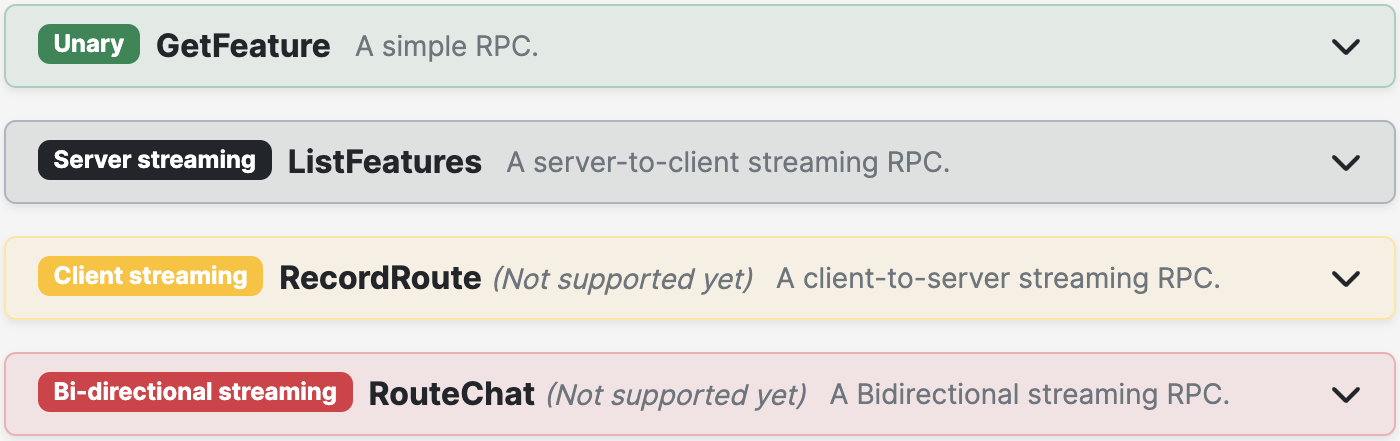
\includegraphics[width=.95\linewidth]{images/testing/screenshots/testing-background-colors}
        \caption{Background colors}
        \label{fig:testing-changes-background-colors}
    \end{subfigure}%
    \begin{subfigure}{.5\textwidth}
        \centering
        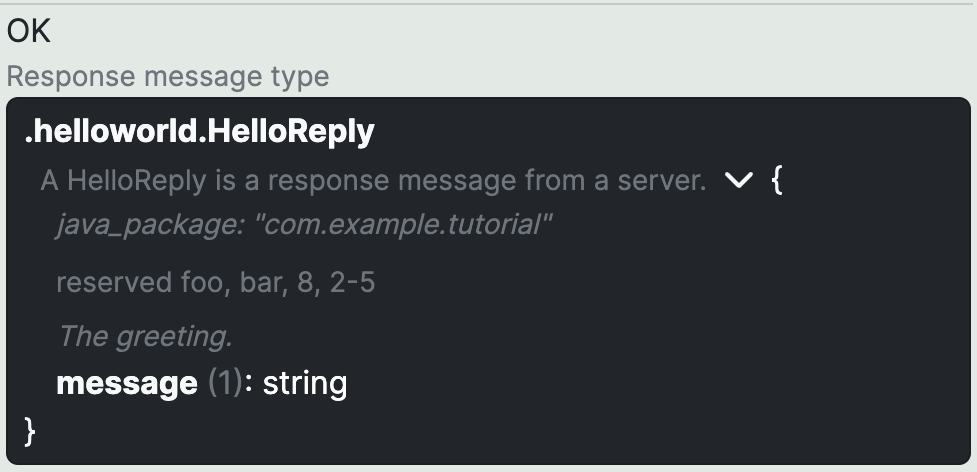
\includegraphics[width=.95\linewidth]{images/testing/screenshots/testing-response-description}
        \caption{Response description}
        \label{fig:testing-changes-response}
    \end{subfigure}%

    \vspace{15mm}%

    \begin{subfigure}{.85\textwidth}
        \centering
        
\includegraphics[width=.95\linewidth]{images/testing/screenshots/testing-cancel}
        \caption{Execute and cancel buttons}
        \label{fig:testing-changes-cancel}
    \end{subfigure}%

    \vspace{15mm}%

    \begin{subfigure}{.85\textwidth}
        \centering
        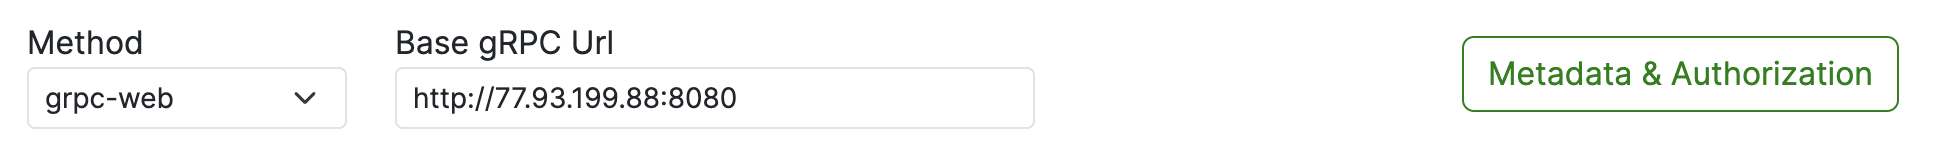
\includegraphics[width=.95\linewidth]{images/testing/screenshots/testing-top-bar}
        \caption{Metadat button, global settings}
        \label{fig:testing-changes-top-bar}
    \end{subfigure}%

    \vspace{15mm}%

    \begin{subfigure}{.45\textwidth}
        \centering
        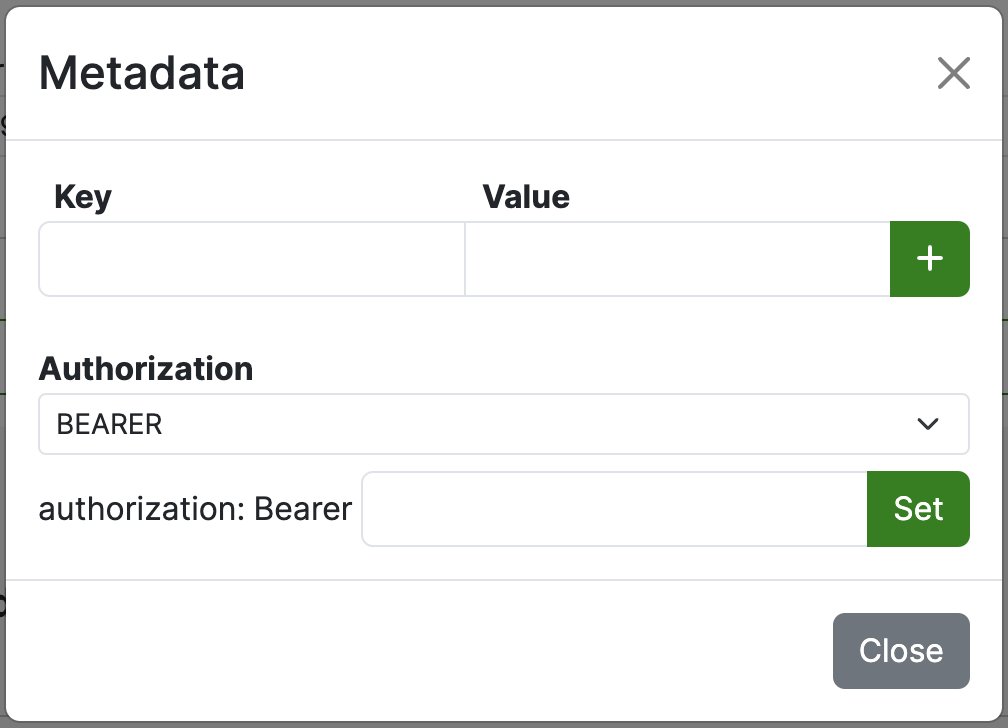
\includegraphics[width=.95\linewidth]{images/testing/screenshots/testing-metadata}
        \caption{Metadata dialog}
        \label{fig:testing-changes-metadata}
    \end{subfigure}%
    \begin{subfigure}{.55\textwidth}
        \centering
        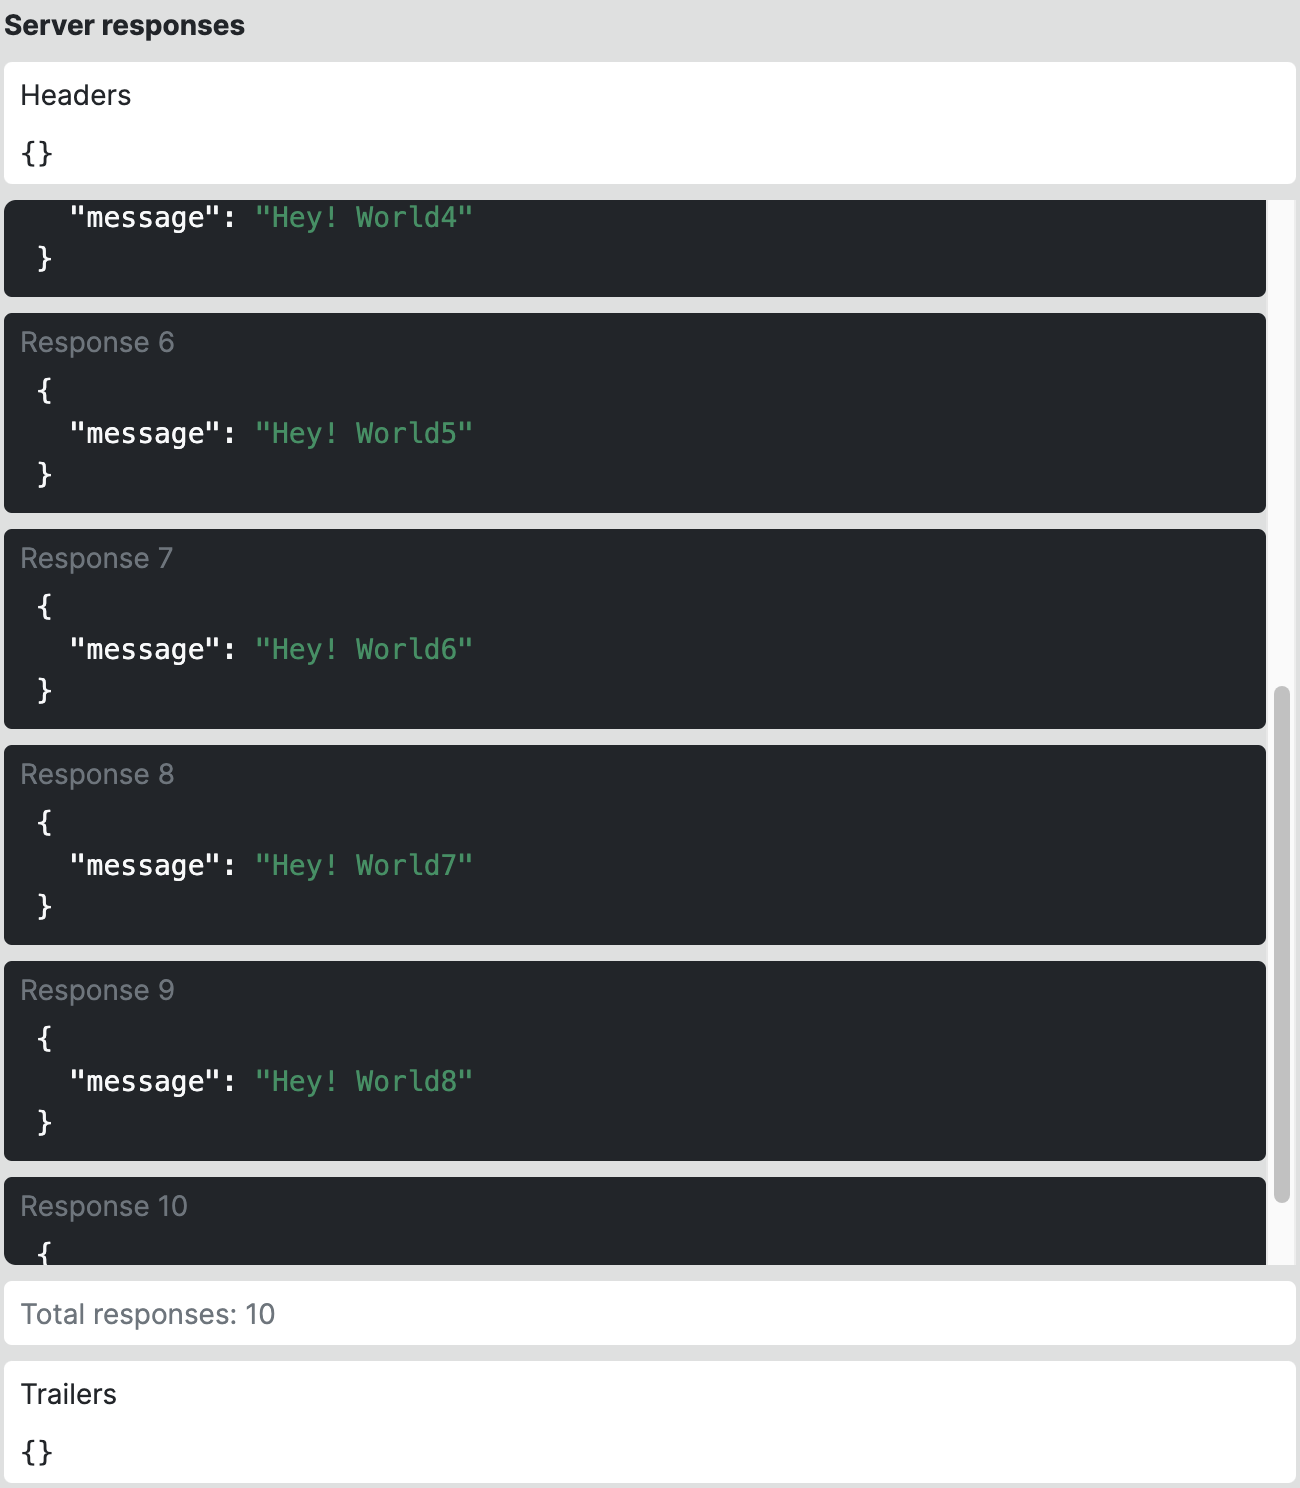
\includegraphics[width=.95\linewidth]{images/testing/screenshots/testing-responses}
        \caption{Scrollable responses with titles and total count}
        \label{fig:testing-changes-responses}
    \end{subfigure}%

    \caption{Changes after testing}
    \label{fig:testing-screenshots}
\end{figure}